\ylDisplay{Jalgrattur} % Ülesande nimi
{EFO žürii} % Autor
{piirkonnavoor} % Voor
{2018} % Aasta
{P 1} % Ülesande nr.
{2} % Raskustase
{
% Teema: Mehaanika

\ifStatement
Graafikul on esitatud jalgratturi kiiruse sõltuvus ajast. Kui suur oli jalgratturi keskmine kiirus kogu sõidu vältel?
\begin{center}
	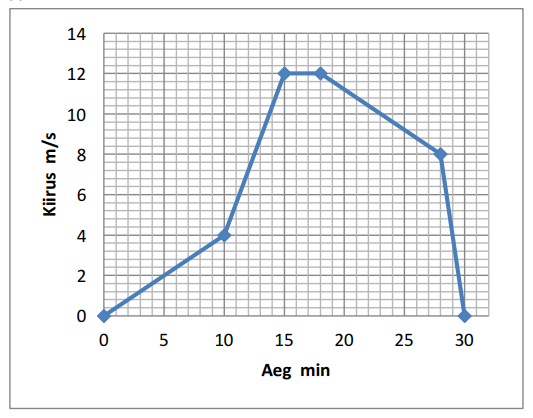
\includegraphics[width=0.5\linewidth]{2018-v2p-01-yl.PNG}
\end{center}
\fi

\ifHint
Keskmine kiirus on kogu teepikkuse ja kogu aja jagatis.
\fi

\ifSolution
Keskmine kiirus on $v_k = \frac{s_{kogu}}{t_{kogu}}$.
Teepikkus on graafku alumine pindala.
Aja saame graafikult. Kuna sõit koosneb viiest etapist, tuleb arvutada iga teepikkus igal etapil.
\begin{center}
$I$ etapp $s_1 = \frac{0 m/s + 4 m/s}{2} \cdot 600s = 1200$ m
\end{center}
\begin{center}
$II$ etapp $s_2 = \frac{4 m/s + 12 m/s}{2} \cdot 300s = 2400$ m
\end{center}
\begin{center}
$III$ etapp $s_3 = 12 m/s \cdot 180s = 2160$ m
\end{center}
\begin{center}
$IV$ etapp $s_4 = \frac{12 m/s + 8 m/s}{2} \cdot 600s = 6000$ m
\end{center}
\begin{center}
$V$ etapp $s_5 = \frac{8 m/s + 0 m/s}{2} \cdot 120s = 480$ m
\end{center}
Kogu teepikkus $s_k = 12 240$ $m$. Keskmine kiirus kogu sõidu vältel
\begin{center}
$v = \frac{12 240 m}{1800s} = 6,8$ m/s
\end{center}
\fi
}
